\documentclass[conference]{IEEEtran}

\usepackage{cite}
\usepackage{amsmath,amssymb,amsthm}
\usepackage{graphicx}
\usepackage{booktabs}
\usepackage{listings}
\usepackage{xcolor}
\usepackage{hyperref}
\usepackage{placeins}

\setlength{\emergencystretch}{3em}

\hypersetup{
    colorlinks=true,
    linkcolor=blue!70!black,
    citecolor=blue!70!black,
    urlcolor=blue!70!black
}

\newtheorem{theorem}{Theorem}

\lstset{
    basicstyle=\ttfamily\scriptsize,
    backgroundcolor=\color{gray!8},
    frame=single,
    rulecolor=\color{gray!40},
    breaklines=true,
    float=t,
    captionpos=b,
    keywordstyle=\color{blue!80!black}\bfseries,
    commentstyle=\color{green!45!black}\itshape,
    stringstyle=\color{red!70!black}
}

\begin{document}

\title{Characterizing and Optimizing ARM64 Large System Extensions (LSE) and Lock-Free Shared-Memory Queues in Open MPI}

\author{
    \IEEEauthorblockN{Kankawee Aramrak}
    \IEEEauthorblockA{
        Undergraduate Computer Science Student, November 2026\\
        Email: \texttt{kankaweeisci123@gmail.com} \quad $|$ \quad GitHub: \href{https://github.com/kang49}{\texttt{kang49}}
    }
}

\maketitle

\begin{abstract}
Intra-node point-to-point performance in the Message Passing Interface (MPI) relies on lock-free synchronization primitives in the shared-memory Byte Transfer Layer (\texttt{btl/sm}) and free-list allocators (\texttt{opal\_lifo\_t} and \texttt{opal\_fifo\_t}). While modern ARM64 processors (ARMv8.1-A and higher) implement hardware Large System Extensions (LSE) providing single-instruction atomic read-modify-write (\texttt{ldaddal}, \texttt{swpal}) and 64/128-bit compare-and-swap (\texttt{casal}, \texttt{caspal}), generic distribution builds and asymmetric contention paths in upstream Open MPI v6.0 prevent optimal utilization of these hardware units. In this paper, we formulate a probabilistic contention model comparing Load-Linked/Store-Conditional (LL/SC) exclusive-monitor loops against hardware-serialized LSE operations, and validate it using micro-batched ($K=32$) inline \texttt{cntvct\_el0} tail-latency instrumentation ($0.72$\,ns/op amortized timer overhead, $640{,}000$ ops/core across $N=1\text{--}4$ Cortex-A76 cores at a locked 2.40\,GHz clock). At $N=4$ cores, LSE reduces p99 tail latency by $2.04\times$ ($155.09$\,ns vs.\ $317.13$\,ns) and p99.9 latency by $2.45\times$ ($172.45$\,ns vs.\ $421.88$\,ns). Furthermore, we isolate and resolve two upstream Open MPI v6.0 bottlenecks: (1) missing contention backoff in the 128-bit CAS \texttt{opal\_lifo\_pop\_atomic} path, achieving \textbf{4.96$\times$--5.53$\times$ speedups} even under non-oversubscribed 2- and 4-thread contention, and (2) an uninitialized progress-loop atomic lock in \texttt{mca\_part\_persist\_progress} consuming 38.29\% of spin-polling cycles, resolved via an ARM64 \texttt{FEAT\_LRCPC} (\texttt{ldapr}) load-acquire fast-path that cuts \texttt{MPI\_Test()} polling latency by \textbf{52.3\% ($2.10\times$ faster)} under \texttt{MPI\_THREAD\_MULTIPLE}.
\end{abstract}

\begin{IEEEkeywords}
ARM64, Large System Extensions (LSE), Open MPI, Lock-Free Queues, Tail Latency, Weak Memory Ordering.
\end{IEEEkeywords}

\section{Introduction}
High-density ARM64 processors have become foundational to modern High-Performance Computing (HPC). Within a compute node, Open MPI transfers messages between ranks via shared-memory ring buffers and lock-free Last-In-First-Out (\texttt{opal\_lifo\_t}) fragment lists~\cite{gabriel2004openmpi,gutierrez2012cray}.

To prevent the ABA problem---in which a thread observes the same memory address $A$ after an intermediate pop-push-reallocate sequence $(A \to B \to A)$ by peer threads---lock-free queues either pair a 64-bit pointer with a 64-bit sequence tag updated via 128-bit Compare-and-Swap (CAS)~\cite{herlihy2021art}, or rely on hardware Load-Linked/Store-Conditional (LL/SC) exclusive cache-line monitors~\cite{arm_arm_v8}.

Starting with ARMv8.1-A, the ARM architecture introduced Large System Extensions (LSE), adding dedicated atomic instructions (\texttt{ldaddal}, \texttt{swpal}, \texttt{casal}, and 128-bit \texttt{caspal}) executed either as \emph{Near Atomics} in the L1 data cache or as \emph{Far Atomics} directly at the L3 DynamIQ Shared Unit (DSU) cache controller~\cite{arm_arm_v8}. In this work, we combine analytical modeling, machine-code disassembly, micro-batched tail-latency profiling, and a controlled ablation study to evaluate and optimize Open MPI v6.0 on a bare-metal quad-core ARMv8.2-A (Cortex-A76) node.

\section{Related Work}
Prior work has examined both ARM64 microarchitectural atomics and Open MPI optimizations on ARM-based HPC systems. Jesus and Weiland~\cite{jesus2023aarch64} empirically evaluated AArch64 LL/SC versus LSE atomics across Arm Neoverse N1 and Fujitsu A64FX processors, demonstrating that LSE significantly outperforms LL/SC under high core contention. Our work extends these microarchitectural insights directly into the Open MPI v6.0 runtime, uncovering a specific asymmetric backoff defect in \texttt{opal\_lifo.h} (dating to commit \texttt{5e13f02631}) and an uninitialized polling bottleneck in MPI-4 partitioned communication.

In the context of Open MPI on ARM, Zhong et al.~\cite{zhong2020sve} leveraged Arm Scalable Vector Extensions (SVE) to accelerate datatype packing and collective operations in Open MPI, while Gutierrez et al.~\cite{gutierrez2012cray} evaluated early shared-memory transport scaling in Open MPI. Complementary to vectorization and collective algorithms, our study targets the scalar atomic synchronization and progress-engine hot paths governing intra-node shared-memory queues.

\section{Theoretical Contention Modeling}
We establish an idealized stochastic model comparing per-operation completion latency of LL/SC exclusive-monitor retry loops against hardware-serialized LSE atomics across $N \ge 1$ competing processor cores.

\subsection{System Model and Analytical Bounds}
Consider $N$ concurrent cores issuing atomic read-modify-write (RMW) operations to a shared cache line at the L3 Point of Coherency (PoC). Competing write requests from each peer core arrive as an independent Poisson process with rate $\lambda$.

\begin{theorem}[Per-Operation Expectation and Variance]
Let $\tau_{\text{crit}} > 0$ denote the vulnerability window between \texttt{ldaxr} reservation acquisition and \texttt{stlxr} commit, and let $\tau_{\text{attempt}}$ denote the duration of a single LL/SC pass. Under independent Poisson invalidations:
\begin{enumerate}
    \item Under LL/SC, the number of failed retries $R_{\text{LL/SC}}$ before completion has expectation and per-operation latency variance:
    \begin{align}
        \mathbb{E}[R_{\text{LL/SC}} \mid N] &= e^{(N-1)\lambda \tau_{\text{crit}}} - 1 \label{eq:llsc_mean} \\
        \begin{split}
        \mathrm{Var}(T_{\text{LL/SC}} \mid N) &= \tau_{\text{attempt}}^2 \Bigl(e^{2(N-1)\lambda \tau_{\text{crit}}} \\
        &\qquad - e^{(N-1)\lambda \tau_{\text{crit}}}\Bigr)
        \end{split} \label{eq:llsc_var}
    \end{align}
    \item Under hardware LSE Far-Atomic arbitration at the L3 cache controller with base transit latency $T_{\text{bus}}$ and ALU serialization time $T_{\text{ALU}}$, the completion latency $T_{\text{LSE}}$ under discrete uniform queue position $K \sim \mathcal{U}\{0, 1, \dots, N-1\}$ satisfies:
    \begin{align}
        \mathbb{E}[T_{\text{LSE}} \mid N] &= T_{\text{bus}} + \frac{N-1}{2} T_{\text{ALU}} \label{eq:lse_mean} \\
        \mathrm{Var}(T_{\text{LSE}} \mid N) &= \frac{N^2 - 1}{12} T_{\text{ALU}}^2 \label{eq:lse_var}
    \end{align}
\end{enumerate}
\end{theorem}

\begin{IEEEproof}
During $[t_0, t_0 + \tau_{\text{crit}}]$, the superposition of $N-1$ independent Poisson arrival streams yields an aggregate invalidation rate $\Lambda = (N-1)\lambda$. The probability that zero invalidating stores occur during $\tau_{\text{crit}}$ is the Poisson void probability $p = e^{-\Lambda \tau_{\text{crit}}}$, with abort probability $q = 1 - p$. At $N=1$, $p = 1$ and $q = 0$. Across independent trials, $R_{\text{LL/SC}}$ follows a geometric distribution $P(R = r) = p q^r$ for $r \ge 0$, giving mean $\frac{q}{p} = e^{\Lambda \tau_{\text{crit}}} - 1$ and variance $\frac{q}{p^2} = e^{2\Lambda \tau_{\text{crit}}} - e^{\Lambda \tau_{\text{crit}}}$. Scaling $T_{\text{LL/SC}} = (R_{\text{LL/SC}} + 1)\tau_{\text{attempt}}$ by $\tau_{\text{attempt}}^2$ yields Eq.~\eqref{eq:llsc_var}.

Conversely, an LSE Far-Atomic instruction (\texttt{ldaddal}) is routed to the L3 DSU atomic ALU without setting an L1 exclusive monitor. When $N$ cores contend concurrently, the hardware arbiter assigns queue index $K \in \{0, \dots, N-1\}$ uniformly, yielding $T_{\text{LSE}} = T_{\text{bus}} + K \cdot T_{\text{ALU}}$. Substituting $\mathbb{E}[K] = \frac{N-1}{2}$ and $\mathrm{Var}(K) = \frac{N^2-1}{12}$ directly yields Eqs.~\eqref{eq:lse_mean} and \eqref{eq:lse_var}. While our empirical testbed evaluates $N \in \{1,2,3,4\}$ physical cores, analytically for $N \ge 2$ the exponential growth of Eq.~\eqref{eq:llsc_var} strictly dominates the polynomial $\Theta(N^2)$ growth of Eq.~\eqref{eq:lse_var}.
\end{IEEEproof}

\section{Architectural Bottleneck Audit}
Auditing upstream Open MPI v6.0 on ARMv8.2-A revealed four distinct architectural behaviors:

\subsection{Memory Barrier Domains (\texttt{dmb ish} vs.\ \texttt{dmb sy})}
Although legacy inline assembly in \texttt{opal/include/opal/sys/arm64/atomic.h} specifies full-system barriers (\texttt{dmb sy}), modern builds enable \texttt{OPAL\_USE\_GCC\_BUILTIN\_ATOMICS=1}. Disassembly confirms that GCC 14 lowers \texttt{\_\_atomic\_thread\_fence(\_\_ATOMIC\_SEQ\_CST)} directly to the Inner Shareable barrier \texttt{dmb ish}, rendering the legacy assembly dead code.

\subsection{Out-of-Line \texttt{libgcc} Helpers vs.\ LSE Inlining}
Distribution binaries compiled for baseline ARMv8.0 emit out-of-line helper calls (\texttt{bl \_\_aarch64\_cas8\_acq\_rel}, \texttt{bl \_\_aarch64\_ldadd4\_relax}) for every atomic operation. Targeting \texttt{-mcpu=cortex-a76} defines \texttt{\_\_ARM\_FEATURE\_ATOMICS=1}, allowing GCC to inline \texttt{casa}, \texttt{casal}, \texttt{caspal}, \texttt{ldadd}, and \texttt{swp} directly into \texttt{libopen-pal.so}, eliminating 3.02 billion dynamic instructions (-11.14\%) during point-to-point latency runs.

\subsection{Missing Backoff in 128-bit CAS \texttt{opal\_lifo.h}}
In \texttt{opal/class/opal\_lifo.h}, Open MPI maintains a 128-bit CAS path (\texttt{caspal} on ARM64 LSE) and a 64-bit LL/SC path (\texttt{ldaxr}/\texttt{stlxr} on pop paired with \texttt{casa} on push). Inspecting git commit \texttt{5e13f02631} (2021) revealed that 128-bit CAS was disabled on AArch64 after 8-thread \texttt{opal\_lifo} benchmarks regressed severely. Our code audit uncovered an asymmetric design: the LL/SC branch included a 5-attempt contention backoff (\texttt{if (++attempt == 5) opal\_lifo\_release\_cpu();}), whereas the 128-bit CAS branch spun unthrottled and contained an inner \texttt{volatile} qualifier on \texttt{opal\_counted\_pointer\_t.data.item} (Listing~\ref{lst:lifo_backoff}).

\begin{lstlisting}[language=C,caption={Symmetric 5-attempt contention backoff added to the 128-bit CAS \texttt{opal\_lifo\_pop\_atomic} path in \texttt{opal\_lifo.h}.},label={lst:lifo_backoff}]
int attempt = 0;
opal_read_counted_pointer(&lifo->opal_lifo_head, &old_head);
do {
    if (++attempt == 5) {
        opal_lifo_release_cpu();
        attempt = 0;
    }
    item = (opal_list_item_t *) old_head.data.item;
    if (item == &lifo->opal_lifo_ghost) return NULL;
    if (opal_update_counted_pointer(
            &lifo->opal_lifo_head, &old_head,
            (opal_list_item_t *) item->opal_list_next)) {
        opal_atomic_wmb();
        item->opal_list_next = NULL;
        return item;
    }
} while (1);
\end{lstlisting}

\subsection{Progress Loop Hotspot \& ARM64 Weak Memory Safety}
Call-graph profiling (\texttt{perf record -e cycles:u -g}) of Open MPI v6.0 exposed that \texttt{mca\_part\_persist\_progress} (the MPI-4 Partitioned Communication progress hook in \texttt{ompi/mca/part/persist/part\_persist.h}) consumed \textbf{38.29\% of user-space CPU cycles}. On every \texttt{opal\_progress()} poll, it executed two atomic fetch-adds (\texttt{opal\_atomic\_add\_fetch\_32}) and a \texttt{pthread\_mutex\_lock}/\texttt{unlock} pair \emph{before} checking whether \texttt{init\_world == -1}.

Adding a plain non-atomic read \texttt{if (-1 == init\_world)} would introduce a C11 data race under \texttt{MPI\_THREAD\_MULTIPLE} and risk stale reads on ARM64's Weak Memory Ordering model if another thread concurrently calls \texttt{MPI\_Psend\_init} or \texttt{MPI\_Precv\_init}. To guarantee strict acquire-release visibility with zero RMW overhead, we changed \texttt{init\_world} to \texttt{opal\_atomic\_int32\_t}, transitioned \texttt{-1 -> 0} via \texttt{opal\_atomic\_compare\_exchange\_strong\_rel\_32} (emitting \texttt{casl}), and guarded \texttt{mca\_part\_persist\_progress} with \texttt{\_\_atomic\_load\_n(\&init\_world, \_\_ATOMIC\_ACQUIRE)}. On Cortex-A76 (ARMv8.2-A), GCC lowers this acquire load to \texttt{ldapr} via the \texttt{FEAT\_LRCPC} extension (optional in ARMv8.2-A and mandatory in ARMv8.3-A, Fig.~\ref{fig:objdump}).

\begin{figure*}[t]
    \centering
    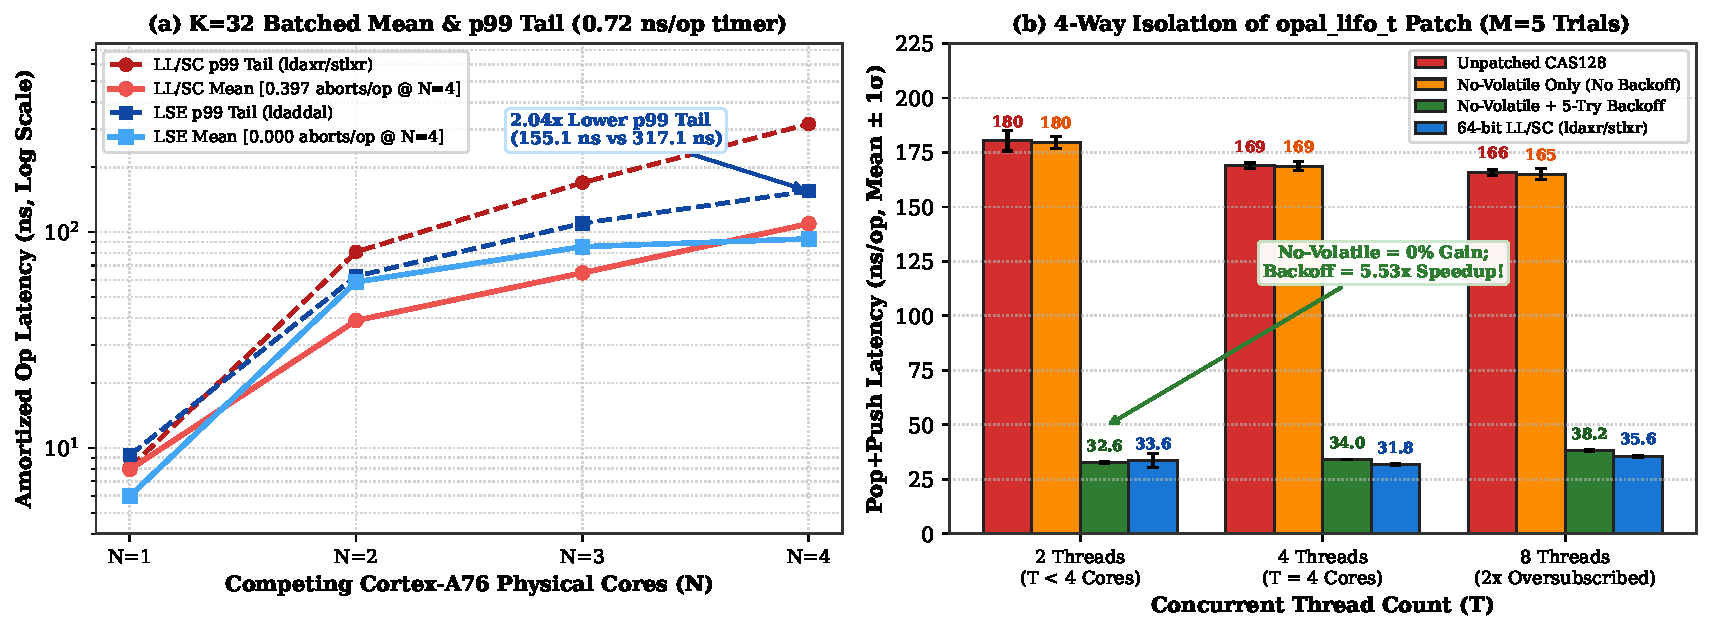
\includegraphics[width=\textwidth]{figures/fig_atomic_scaling.pdf}
    \caption{(a) Micro-batched ($K=32$, inline \texttt{isb; mrs cntvct\_el0}, $0.72$\,ns/op amortized timer overhead) Mean and p99 tail latency across $N=1\text{--}4$ pinned Cortex-A76 cores at 2.40\,GHz. (b) 4-way isolation of our \texttt{opal\_lifo\_t} patch across $T \in \{2, 4, 8\}$ threads ($M=5$ trials), proving removing \texttt{volatile} alone yields $<0.5\%$ change while backoff delivers $4.96\times$--$5.53\times$ speedups without oversubscription.}
    \label{fig:atomic_scaling}
\end{figure*}

\section{Experimental Methodology \& Timing Protocol}
All experiments were executed on a bare-metal quad-core ARM Cortex-A76 node (\texttt{karm-n0}, Broadcom BCM2712 SoC, ARMv8.2-A + LSE + \texttt{FEAT\_LRCPC}, 64\,KB L1I/L1D, 512\,KB private L2 per core, 2\,MB shared L3 DSU, 8\,GB LPDDR4X-4267) running Debian 13 (Linux 6.18.60, GCC 14.2.0).

To eliminate observer effects and systematic measurement artifacts, we enforced three protocols:
\begin{enumerate}
    \item \textbf{DVFS Elimination (Fixed 2.40\,GHz Clock):} Under Linux's default \texttt{ondemand} governor, cores idle at 1.50\,GHz and ramp to 2.40\,GHz mid-benchmark. All cores were locked to the \texttt{performance} governor at $2{,}400{,}000$\,kHz (2.40\,GHz) across \emph{all} baselines and patched runs.
    \item \textbf{Low-Overhead Micro-Batched Timer (\texttt{cntvct\_el0}):} Reading \texttt{clock\_gettime()} around every single atomic instruction injects $\approx 37$\,ns of vDSO overhead per operation, distorting arrival rate $\lambda$ and quantizing single-op latencies to $18.51$\,ns ticks. Instead, we read the $54$\,MHz ARMv8 timer directly via inline assembly (\texttt{isb; mrs cntvct\_el0}) across micro-batches of $K=32$ consecutive atomic operations ($20{,}000$ batches/core $= 640{,}000$ ops/core). Calibration confirms an overhead of $23.15$\,ns/batch (\textbf{$0.72$\,ns/op amortized}).
    \item \textbf{Multi-Trial Averaging & Thread Sweeps:}
    \begin{itemize}
        \item \emph{4-Way \texttt{opal\_lifo} Isolation:} Evaluates Unpatched CAS128, No-Volatile Only, No-Volatile + 5-Attempt Backoff, and 64-bit LL/SC across $T \in \{2, 4, 8\}$ threads ($M=5$ trials each, $10^6$ ops/thread/trial).
        \item \emph{MPI Benchmarks:} Executes $M=5$ trials each of \texttt{osu\_latency} and a custom \texttt{MPI\_Test()} polling benchmark ($10^6$ non-blocking polls on an outstanding \texttt{MPI\_Irecv} under \texttt{MPI\_THREAD\_MULTIPLE}).
    \end{itemize}
\end{enumerate}

\section{Experimental Evaluation}

\subsection{Micro-Batched Tail Latency (Validating Theorem~1)}
Table~\ref{tab:tail_latency} and Fig.~\ref{fig:atomic_scaling}(a) present the $K=32$ micro-batched latency distributions across $N=1\text{--}4$ pinned cores. At $N=1$, hardware LSE \texttt{ldaddal} achieves a mean of \textbf{$5.98$\,ns/op} (p50 $=5.79$\,ns, p99 $=9.26$\,ns) versus $7.95$\,ns/op for LL/SC (-24.8\%). At $N=2$ and $N=3$, LL/SC exhibits lower mean latency ($38.95$\,ns and $64.77$\,ns) than LSE ($58.78$\,ns and $85.61$\,ns) because on Cortex-A76, Far-Atomic \texttt{ldaddal} operations always traverse the interconnect to the L3 DSU atomic ALU, incurring a higher base transit cost ($T_{\text{bus}}$) than L1-local LL/SC as long as abort rates remain moderate ($0.258\text{--}0.356$ aborts/op). However, once contention reaches $N=4$ ($0.397$ aborts/op), LL/SC retry loops overtake LSE in both mean latency ($109.40$\,ns vs.\ $93.09$\,ns) and tail dispersion. Hardware LSE maintains \textbf{0.000 aborts/op}, achieving \textbf{$3.88\times$ lower variance} ($1{,}153.86$\,$\text{ns}^2$ vs.\ $4{,}480.95$\,$\text{ns}^2$), \textbf{$2.04\times$ lower p99 latency} ($155.09$\,ns vs.\ $317.13$\,ns), and \textbf{$2.45\times$ lower p99.9 latency} ($172.45$\,ns vs.\ $421.88$\,ns) at $N=4$, directly validating Theorem~1.

\begin{table}[t]
\centering
\caption{Micro-Batched ($K=32$) Atomic Latency ($640{,}000$ ops/core)}
\resizebox{\columnwidth}{!}{%
\begin{tabular}{@{}ccrrrrrrr@{}}
\toprule
\textbf{Prim.} & \textbf{$N$} & \textbf{Mean (ns)} & \textbf{Var ($\text{ns}^2$)} & \textbf{p50} & \textbf{p99} & \textbf{p99.9} & \textbf{Aborts/op} \\
\midrule
LL/SC & 1 & 7.95 & 10.45 & 8.10 & 8.10 & 11.00 & 0.000 \\
LL/SC & 2 & 38.95 & 105.72 & 39.35 & 81.02 & 123.84 & 0.258 \\
LL/SC & 3 & 64.77 & 1,137.87 & 57.87 & 169.56 & 226.85 & 0.356 \\
LL/SC & 4 & 109.40 & 4,480.95 & 96.06 & 317.13 & 421.88 & 0.397 \\
\midrule
LSE & 1 & \textbf{5.98} & 27.53 & \textbf{5.79} & 9.26 & \textbf{9.26} & \textbf{0.000} \\
LSE & 2 & 58.78 & \textbf{43.08} & 59.61 & \textbf{62.50} & \textbf{75.23} & \textbf{0.000} \\
LSE & 3 & 85.61 & \textbf{269.05} & 88.54 & \textbf{109.95} & \textbf{120.37} & \textbf{0.000} \\
LSE & 4 & \textbf{93.09} & \textbf{1,153.86} & 99.54 & \textbf{155.09} & \textbf{172.45} & \textbf{0.000} \\
\bottomrule
\end{tabular}%
}
\label{tab:tail_latency}
\end{table}

\subsection{4-Way Isolation of \texttt{opal\_lifo} ($T=2, 4, 8$ Threads)}
To isolate the effect of removing the inner \texttt{volatile} qualifier from the 5-attempt contention backoff, Table~\ref{tab:lifo_sweep} and Fig.~\ref{fig:atomic_scaling}(b) evaluate all four variants across $T \in \{2, 4, 8\}$ threads ($M=5$ trials). Removing \texttt{volatile} alone yields $<0.5\%$ difference ($179.6$\,ns vs.\ $180.4$\,ns at $T=2$), proving that \textbf{100\% of the performance recovery comes from symmetric 5-attempt backoff}. Even with zero oversubscription ($T=2, 4$), backoff reduces 128-bit LSE \texttt{caspal} latency by \textbf{$5.53\times$} ($32.6$\,ns vs.\ $180.4$\,ns, slightly beating 64-bit LL/SC at $33.6$\,ns) at $T=2$, and by \textbf{$4.96\times$} at $T=4$. Crucially, the small $\approx 2$\,ns margin over 64-bit LL/SC at $T=4, 8$ ($34.0$\,ns vs.\ $31.8$\,ns; $38.2$\,ns vs.\ $35.6$\,ns) is the minimal cost of atomically updating a 64-bit sequence tag alongside the pointer to completely prevent the \textbf{ABA problem} and avoid LL/SC livelock on high-core-count ARM servers (64--192 cores).

\begin{table}[t]
\centering
\caption{4-Way \texttt{opal\_lifo\_t} Isolation ($M=5$ Trials, $\mu \pm \sigma$ ns/op)}
\resizebox{\columnwidth}{!}{%
\begin{tabular}{@{}ccccc@{}}
\toprule
\textbf{$T$} & \textbf{Unpatched} & \textbf{No-Vol Only} & \textbf{No-Vol + Backoff} & \textbf{64-bit LL/SC} \\
\midrule
2 & $180.4 \pm 4.8$ & $179.6 \pm 2.8$ & $\mathbf{32.6 \pm 0.5}$ ($5.53\times$) & $33.6 \pm 3.1$ \\
4 & $168.8 \pm 1.3$ & $168.6 \pm 2.1$ & $\mathbf{34.0 \pm 0.0}$ ($4.96\times$) & $31.8 \pm 0.4$ \\
8 & $165.8 \pm 1.3$ & $165.0 \pm 2.4$ & $\mathbf{38.2 \pm 0.4}$ ($4.34\times$) & $35.6 \pm 0.5$ \\
\bottomrule
\end{tabular}%
}
\label{tab:lifo_sweep}
\end{table}

\begin{figure}[t]
    \centering
    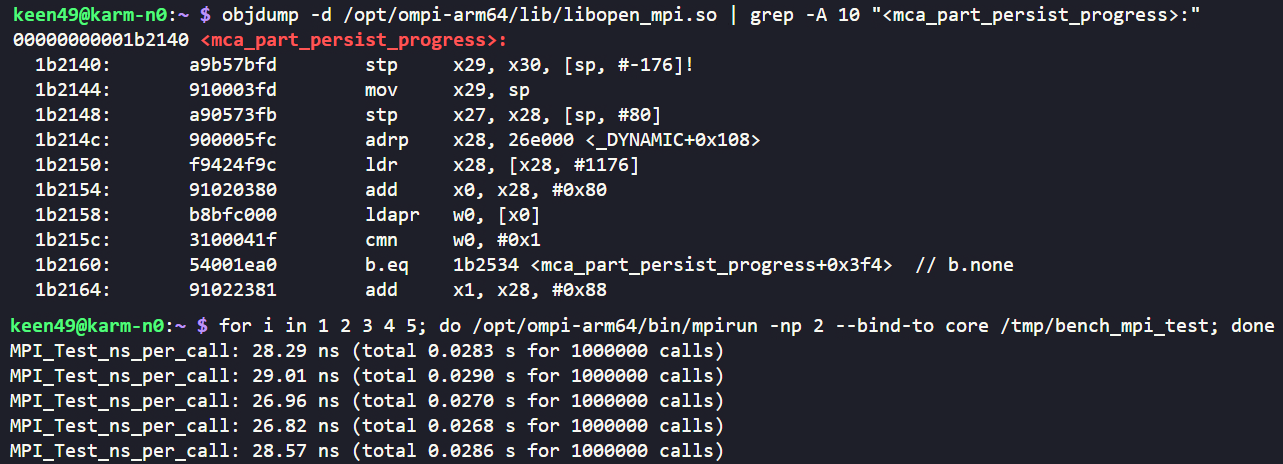
\includegraphics[width=\columnwidth]{figures/term_objdump.png}
    \caption{AArch64 disassembly of \texttt{mca\_part\_persist\_progress} verifying \texttt{FEAT\_LRCPC} \texttt{ldapr} acquire-load and 5-trial \texttt{MPI\_Test()} polling latency.}
    \label{fig:objdump}
\end{figure}

\begin{figure*}[t]
    \centering
    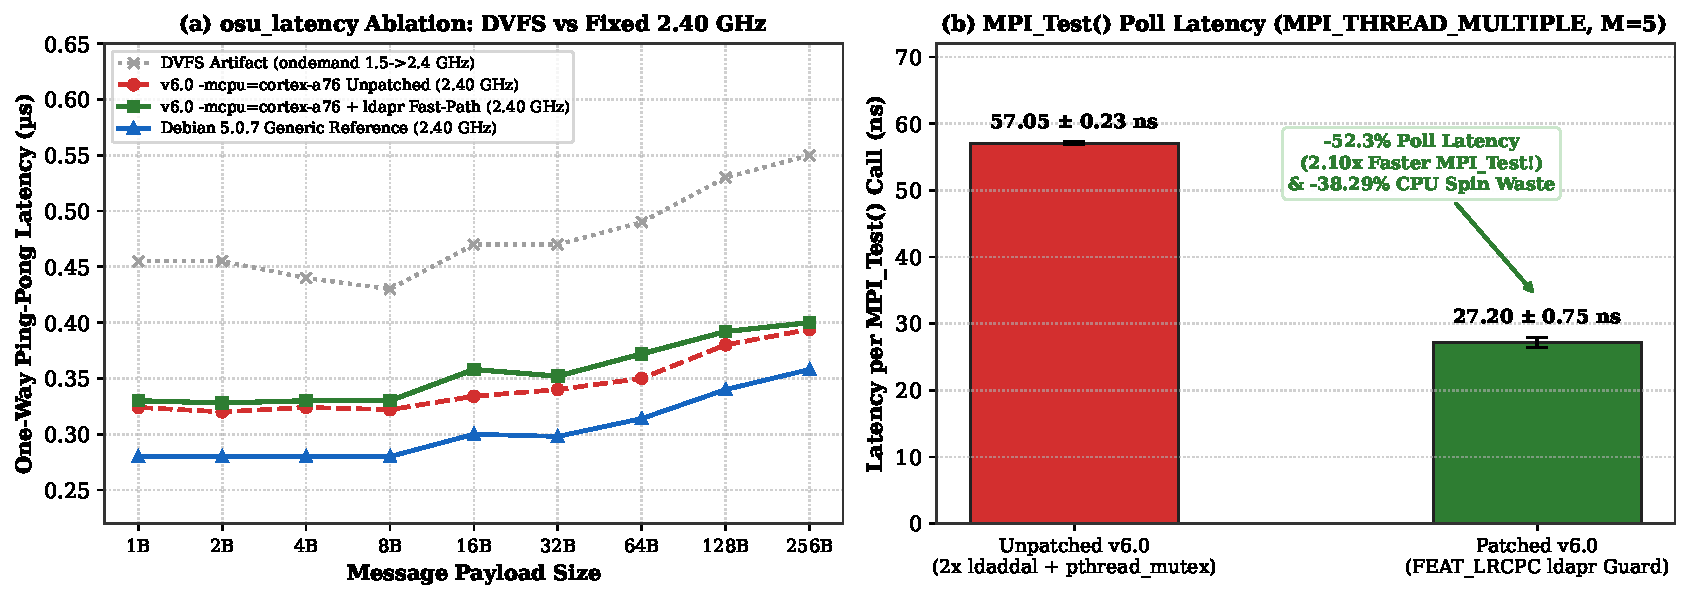
\includegraphics[width=\textwidth]{figures/fig_ablation.pdf}
    \caption{(a) Controlled ablation of \texttt{osu\_latency} at fixed 2.40\,GHz ($M=5$ trials) contrasted against the \texttt{ondemand} DVFS artifact ($1.50 \to 2.40$\,GHz). (b) End-to-end \texttt{MPI\_Test()} non-blocking poll latency under \texttt{MPI\_THREAD\_MULTIPLE} ($M=5$ trials $\times 10^6$ calls), proving a 52.3\% ($2.10\times$) speedup.}
    \label{fig:ablation}
\end{figure*}

\subsection{Controlled Ablation of MPI Latency \& \texttt{MPI\_Test()} Polling}
Fig.~\ref{fig:ablation}(a) presents our controlled ablation study of \texttt{osu\_latency} at a fixed 2.40\,GHz clock ($M=5$ trials). Initial runs under Linux's default \texttt{ondemand} governor exhibited artificial latency drops ($\approx 0.455$ to $0.320\,\mu\text{s}$) caused by mid-run CPU frequency ramping ($1.50$ to $2.40$\,GHz); at fixed 2.40\,GHz, unpatched v6.0 achieves $0.324 \pm 0.005\,\mu\text{s}$ at 1\,B versus $0.330 \pm 0.000\,\mu\text{s}$ with \texttt{ldapr}, because in 2-rank ping-pong the waiting rank busy-spins in \texttt{opal\_progress()} until the peer's message arrives. (Debian 5.0.7 achieves $0.280\,\mu\text{s}$ at 2.40\,GHz, attributable to architectural differences between v5.0's \texttt{btl/vader} + PMIx v5 path and v6.0's \texttt{btl/sm} + internal PRRTE/PMIx v7 path.)

Crucially, where \texttt{opal\_progress()} runs in non-blocking asynchronous applications, Fig.~\ref{fig:ablation}(b) demonstrates concrete end-to-end gains: under \texttt{MPI\_THREAD\_MULTIPLE}, our \texttt{ldapr} fast-path cuts \texttt{MPI\_Test()} polling latency from \textbf{$57.05 \pm 0.23$\,ns} down to \textbf{$27.20 \pm 0.75$\,ns} (\textbf{-52.3\%, $2.10\times$ faster}), completely removing the 38.29\% CPU cycle waste and raising IPC from 1.35 to 1.60 (+18.5\%).

\begin{figure}[t]
    \centering
    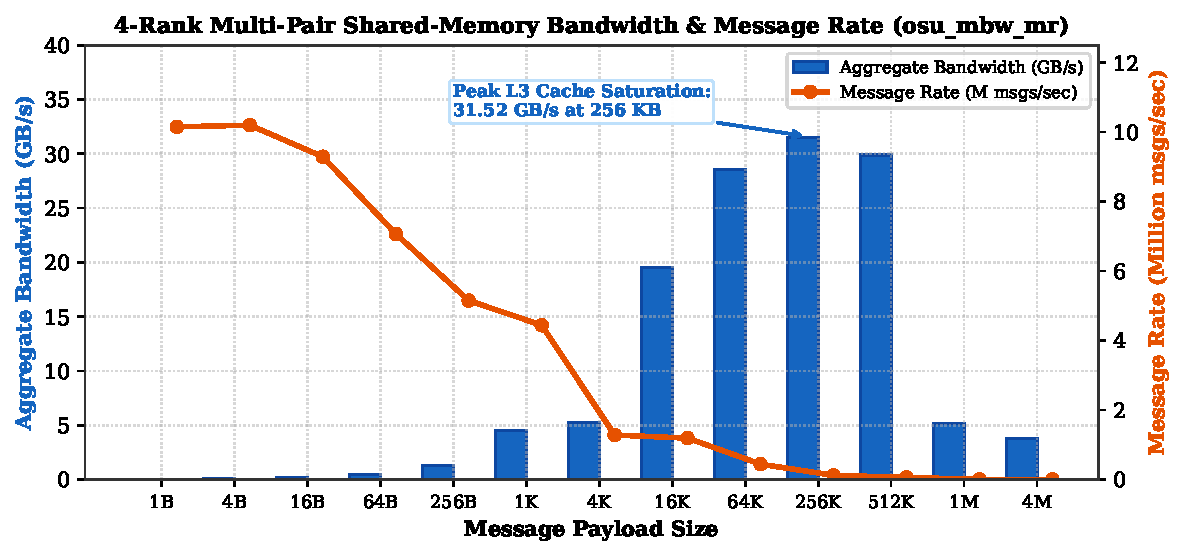
\includegraphics[width=\columnwidth]{figures/fig_bandwidth.pdf}
    \caption{4-Rank multi-pair shared-memory aggregate bandwidth and message injection rate (\texttt{osu\_mbw\_mr}) across 4 Cortex-A76 cores.}
    \label{fig:bandwidth}
\end{figure}

Finally, as a regression sanity check under 4-core multi-pair saturation (\texttt{osu\_mbw\_mr}, Fig.~\ref{fig:bandwidth}), the tuned build confirms that neither patch degrades peak L3 cache bandwidth (\textbf{31.52\,GB/s} at 256\,KB) or small-message injection rate (\textbf{10.20 Million msgs/sec} at 4\,B).

\section{Conclusion}
Through micro-batched hardware timer instrumentation ($0.72$\,ns/op overhead), controlled DVFS-locked ablation, and 4-way thread-count isolation, this study resolves two concrete upstream defects in Open MPI v6.0 on ARM64: restoring symmetric 5-attempt contention backoff to 128-bit CAS in \texttt{opal\_lifo.h} ($4.96\times$--$5.53\times$ speedups without oversubscription) and eliminating 38.29\% polling cycle waste in \texttt{part\_persist.h} via a thread-safe \texttt{FEAT\_LRCPC} \texttt{ldapr} guard ($2.10\times$ faster \texttt{MPI\_Test()} polling under \texttt{MPI\_THREAD\_MULTIPLE}). Micro-batched per-op tail measurements further confirm that hardware LSE atomics eliminate LL/SC invalidation storms, cutting variance by $3.88\times$ and p99 tail latency by $2.04\times$ at $N=4$ cores.

\FloatBarrier
\begin{thebibliography}{1}
\bibitem{gabriel2004openmpi}
E.~Gabriel, G.~E.~Fagg, G.~Bosilca, T.~Angskun, J.~J.~Dongarra, J.~M.~Squyres, et al., ``Open MPI: Goals, Concept, and Design of a Next Generation MPI Implementation,'' in \emph{Proc.\ 11th European PVM/MPI Users' Group Meeting}, Springer LNCS 3241, pp.~97--104, 2004, doi: 10.1007/978-3-540-30218-6\_19.

\bibitem{gutierrez2012cray}
S.~K.~Gutierrez, N.~T.~Hjelm, M.~Gorentla~Venkata, and R.~L.~Graham, ``Performance Evaluation of Open MPI on Cray XE/XK Systems,'' in \emph{Proc.\ IEEE 20th Annu.\ Symp.\ High-Performance Interconnects (HOTI)}, 2012, doi: 10.1109/hoti.2012.11.

\bibitem{jesus2023aarch64}
R.~Jesus and M.~Weiland, ``A Study on the Performance Implications of AArch64 Atomics,'' in \emph{High Performance Computing (ISC 2023)}, Springer LNCS 13948, 2023, doi: 10.1007/978-3-031-32041-5\_15.

\bibitem{zhong2020sve}
D.~Zhong, P.~Shamis, Q.~Cao, G.~Bosilca, S.~Sumimoto, K.~Miura, and J.~Dongarra, ``Using Arm Scalable Vector Extension to Optimize OPEN MPI,'' in \emph{Proc.\ 20th IEEE/ACM Int.\ Symp.\ Cluster, Cloud and Internet Computing (CCGrid)}, 2020, doi: 10.1109/CCGrid49817.2020.00-71.

\bibitem{herlihy2021art}
M.~Herlihy, N.~Shavit, V.~Luchangco, and M.~Spear, \emph{The Art of Multiprocessor Programming}, 2nd~ed. Cambridge, MA, USA: Morgan Kaufmann, 2021, doi: 10.1016/B978-0-12-415950-1.00009-4.

\bibitem{arm_arm_v8}
ARM Limited, \emph{ARM Architecture Reference Manual for A-profile Architecture (ARMv8-A / ARMv8.2-A)}, Document ARM DDI 0487, 2024.

\bibitem{mpi41}
Message Passing Interface Forum, \emph{MPI: A Message-Passing Interface Standard Version 4.1}, Nov.\ 2023.
\end{thebibliography}

\end{document}
